 % $Rev: 799 $
% $LastChangedDate: 2011-05-24 14:07:56 +0200 (Di, 24 Mai 2011) $ 
% $Author: meesters $ 
\documentclass[a4paper, 11pt, twoside, openany, titlepage, dvipsnames]{book}
\usepackage[english]{babel}
\usepackage[utf8]{inputenc}
\usepackage{caption} %for captions
\usepackage[T1]{fontenc}
\usepackage{graphicx}
\usepackage{amsfonts, amsmath, amssymb}
\usepackage{fancyhdr}
\usepackage{float}
% page layout with the geometry package
\usepackage[margin=1.0in, centering]{geometry}
% changing line pitch
\usepackage{setspace}
% for floating text around an image
\usepackage{wrapfig}
% for arbitrarily enumerated lists
\usepackage{enumerate}
% natbib
\usepackage{natbib}
% color names
\usepackage[usenames]{xcolor}
% for colored headings
\usepackage{titlesec}
% for colored table segments
\usepackage{colortbl}
% additional symbols
\usepackage{marvosym}
\newcommand{\alert}[1]{{\centering\fbox{\parbox{0.98\linewidth}{\noindent {\huge\color{Red}\Stopsign}\bfseries #1}}}}
\newcommand{\alertv}[1]{{\centering\fbox{\parbox{0.98\linewidth}{\noindent {\huge\color{Red}\Stopsign} #1}}}}

\usepackage{listings}
\lstloadlanguages{Python,bash,C++}
\lstset{showspaces=false,
basicstyle=\small,
showstringspaces=false}

\definecolor{pblue}{RGB}{45,106,148}
\definecolor{pdarkblue}{RGB}{35,71,100}
\definecolor{plightblue}{RGB}{90,159,212}
\definecolor{pyellow}{RGB}{255,212,59}
\definecolor{pdarkyellow}{RGB}{255,188,41}
\definecolor{plightyellow}{RGB}{255,232,115}
\definecolor{pdarkgrey}{RGB}{100,100,100}
\definecolor{pgrey}{RGB}{153,153,153}
\definecolor{plightgrey}{RGB}{233,233,233}
\definecolor{plightgrey2}{RGB}{247,247,247}
\definecolor{pnavy}{RGB}{0,0,170}
\definecolor{BrickRed}{RGB}{150,22,11}
\definecolor{BlueViolet}{RGB}{138, 43, 226}
\definecolor{PineGreen}{RGB}{0, 51, 0}
\definecolor{light-gray}{gray}{0.95}

\titleformat{\chapter}[display]
{\color{pdarkblue}\normalfont\huge\bfseries}{\chaptertitlename\
\thechapter}{20pt}{\Huge}

\titleformat{\section}
{\color{pdarkblue}\normalfont\Large\bfseries}{\thesection}{1em}{}

\titleformat{\subsection}
{\color{pdarkblue}\normalfont\large\bfseries}{\thesubsection}{1em}{}

\titleformat{\subsubsection}
{\color{pdarkblue}\normalfont\bfseries}{\thesubsubsection}{1em}{}

%default python listings:
\lstdefinestyle{Python}
{
  language=Python,
  basicstyle=\small,
  showstringspaces=false,
  stepnumber=5,
  numberstyle=\tiny,
  numbersep=5pt,
  showspaces=false,
  frame=single,
  framerule=0.4pt,
  rulecolor=\color{pgrey},
  backgroundcolor=\color{white},
  stringstyle=\color{BrickRed},
  keywordstyle=\color{BlueViolet}\bfseries,
  commentstyle=\color{PineGreen}\bfseries,
  identifierstyle={},
  emph={[10]self}, emphstyle={[10]\color{pblue}},
  emph={[11]yield}, emphstyle={[11]\color{pblue}},
}

%default python listings:
\lstdefinestyle{C++}
{
  language=C++,
  basicstyle=\small,
  showstringspaces=false,
  stepnumber=5,
  numberstyle=\tiny,
  numbersep=5pt,
  showspaces=false,
  frame=single,
  framerule=0.4pt,
  rulecolor=\color{pgrey},
  backgroundcolor=\color{white},
  stringstyle=\color{BrickRed},
  keywordstyle=\color{BlueViolet}\bfseries,
  commentstyle=\color{PineGreen}\bfseries,
  identifierstyle={},
  emph={[10]self}, emphstyle={[10]\color{pblue}},
  emph={[11]yield}, emphstyle={[11]\color{pblue}},
}

%default shell listings:
\lstdefinestyle{Shell}
{
  language=Bash,
  basicstyle=\ttfamily\small,
  showstringspaces=false,
  frame=single,
  framerule=0.4pt,
  rulecolor=\color{pgrey},
  backgroundcolor=\color{plightgrey2},
  stringstyle=\color{black},
  keywordstyle=\color{black},
  commentstyle=\color{black}\bfseries,
  identifierstyle=\color{black},
  emph={[10]\$,>>>}, emphstyle={[10]\color{pblue}}
}

%default plain listings (e.g. for config files):
\lstdefinestyle{Plain}
{ 
  stepnumber=5,
  numberstyle=\tiny,
  numbersep=5pt,
  language=Bash,
  basicstyle=\ttfamily\small,
  showstringspaces=false,
  frame=single,
  framerule=0.4pt,
  rulecolor=\color{pgrey},
  backgroundcolor=\color{plightgrey2},
  stringstyle=\color{black},
  keywordstyle=\color{black},
  commentstyle=\color{blue}\bfseries,
  identifierstyle=\color{black},
  emph={[10]\$,>>>}, emphstyle={[10]\color{pblue}}
}

\definecolor{UrlColor}{rgb}{0,0.08,0.45}

%\usepackage{algorithm}
%\usepackage{algpseudocode}

%\def\pgfsysdriver{pgfsys-dvipdfm.def} % to explicitly load the driver before tikz
\usepackage{tikz}
\usetikzlibrary{arrows,shapes,backgrounds,positioning,shadows,decorations}

% turn on numbering on any level
\setcounter{secnumdepth}{10}
% turn on numbering up to \subsubsection in the toc, too
\setcounter{tocdepth}{3}

\usepackage[pdftex,pdfpagelabels,plainpages=false,pdfborder={0 0 0}]{hyperref}
% metadata
\hypersetup{
pdfauthor = {Christian Meesters},
pdftitle = {YAMAS -- Meta-Analysis from the University of Bonn},
pdfsubject = {Meta-Analysis},
pdfkeywords = {Meta-Analysis},
pdfcreator = {LaTeX with hyperref package},
pdfproducer = {pdflatex}}

\usepackage[scaled]{helvet}
\renewcommand*\familydefault{\sfdefault}

\author{Christian Meesters}

\begin{document}
\pagestyle{fancyplain}
\addtolength{\headheight}{\baselineskip}
\renewcommand{\chaptermark}[1]{\markboth{#1}{}}
\renewcommand{\sectionmark}[1]{\markright{\thesection\ #1}}
\lhead[\fancyplain{}{\thepage}]{\fancyplain{}{\rightmark}}
\rhead[\fancyplain{}{\leftmark}]{\fancyplain{}{\thepage}}
\cfoot{}

% $Rev: 831 $
% $LastChangedDate: 2011-11-25 13:28:29 +0100 (Fr, 25 Nov 2011) $ # date of last revision
% $Author: meesters $ # author of the last revision
% Christian Meesters" # main author / original author

\thispagestyle{empty}
\newcommand{\Rule}{\rule{\textwidth}{1mm}}
\begin{center}
\Rule\vspace{5mm}
\sffamily\bfseries\LARGE

YAMAS \\
-- \\
Yet Another Meta-Analysis Software
\vspace{1mm}\Rule
\vfill
Christian Meesters\\
Markus Leber\\
Christine Herold\\
Manuel Mattheisen\\
Dmitriy Drichel\\
André Lacour\\
Tim Becker\\
\vfill
Deutsches Zentrum für Neurodegenerative Erkrankungen (DZNE)\\
German Centre for Neurodegenerative Diseases\\
Outstation Bonn
\vfill
Institute for Medical Biometrics, Informatics and Epidemiology (IMBIE)\\
University of Bonn

\vspace{2cm}

\hfill
\vfill
\small Bonn, \today
\end{center}

\pagenumbering{roman}
% Remove parskip for toc
\setlength{\parskip}{0ex plus 0.5ex minus 0.2ex}
\tableofcontents
\pagenumbering{arabic}
% $Rev: 935 $
% $LastChangedDate: 2014-06-17 22:08:43 +0200 (Di, 17 Jun 2014) $ 
% $Author: meesters $ 
\chapter{Introduction}

Welcome to \textsc{yamas} (\textcolor{pdarkblue}{\bf Y}et \textcolor{pdarkblue}{A}nother \textcolor{pdarkblue}{M}eta-\textcolor{pdarkblue}{A}nalysis \textcolor{pdarkblue}{S}oftware)!\newline

\textsc{yamas} tries to fulfill various meta-analysis needs with regard to genome-wide association studies. There are other softwares around, but we hope with \textsc{yamas} more features are provided and more possible pitfalls avoided.\newline

This manual should provide you with a comprehensive overview of the software. Still, if after referring to this manual a nagging question is left (or, if you discover a bug), you are most welcome to write us \Email{Tim.Becker@dzne.de} and \Email{meesters@uni-mainz.de}\footnote{I left the institute shortly after writing the software and am now to find at the \textsc{zdv}, University of Mainz, Germany (see \url{http://zdv.uni-mainz.de}).}(please put both emails in the address field of your mail client) in case of any nagging question.\newline

Note that you can \textcolor{pdarkblue}{\bf click on every link to jump within this manual}.\newline

In order to get started we recommend reading at least the following chapter. For the rest skip whatever you like, but be aware that you might miss essential information which you need to exploit the full power of \textsc{yamas}.\newline

\textbf{\Huge Enjoy!}







% $Rev: 925 $
% $LastChangedDate: 2012-09-10 16:19:51 +0200 (Mo, 10 Sep 2012) $
% $Author: meesters $
\chapter[Usage]{Using \textsc{yamas}}

First things first: This chapter shows several examples on the shell. Parameters given in angular brackets (e.\,g. \texttt{[parameter]}) are optional, required arguments are shown as \texttt{<arguments>}.

Sometimes commands did not fit in one line. In this case you might see a backslash (\verb+\+) to indicate a line break. You may or may not copy this to your command shell - it doesn't matter for all shells known to us.

\section{Defining Input}

Input may be defined using the command line or a configuration file. However, not all arguments can be given using both interfaces.

\subsection{The Commandline}

Command line arguments are given as follows:

\begin{lstlisting}[style=shell]
$ yamas -t 4
$ # or
$ yamas --threads 4
\end{lstlisting}

Options usually come with a short (\verb+-+) and a long (\verb+--+), more verbose, version. You may choose, they are equivalent. However, some options are short or long, only. The following table shows a complete list of options.

And you may ask \textsc{yamas} for help, if you like:
\begin{lstlisting}[style=shell]
$ yamas -h
$ # or
$ yamas --help
\end{lstlisting}
A full list of possible command line options is given along with their defaults.\\

\begin{table}[H]
 \caption{\emph{List of available command line options.} A detailed description for some is given below.}
 \centering
 \label{usage:table:commandline_options}
\begin{tabular}{p{3cm}p{7cm}p{4cm}}
\rowcolor{light-gray}Option & Description & Reference\\\hline
\verb+-t+, \verb+--threads+ & gives the number of threads to use for parallel algorithms  & see paragraph \ref{usage:op:threading}\\
\verb+-c+, \verb+--config+  & specifies path to the configuration file                    & see paragraph \ref{usage:op:configfile}\\
\verb+-l+, \verb+--logfile+ & specifies name of the log file \textsc{yamas} produces -- this is also the major output file
                                                                                          & see paragraph \ref{usage:op:logfile}\\
\verb+-a+, \verb+--algo+    & specifies the algorithm to perform                          & see paragraph \ref{usage:op:algorithms}\\
\verb+--odds_ratio+         & whether or not \textsc{yamas} is dealing with odds ratios, default is no & --- \\
\verb+-v+, \verb+--verbose+  & if set, \textsc{yamas} will behave a little more verbose   & see paragraph \ref{usage:op:verbosity}\\
\verb+ --cl+		    & set confidence level for confidence intervals (default value: 0.95) & see paragraph \ref{usage:output} \\
\verb+-p+, \verb+--pthreshold+ & only markers with combined P-vlalues $\leq$ this threshold will be written to the log file & ---\\
\verb+--r2threshold+        & only proxy SNPs with an mutual r$^2 \geq$ this threshold will be considered & see paragraph \ref{algo:fillwithproxies}\\
\verb+--chromosome+         & can be used to select a specific chromosome to be analysed, only & see paragraph \ref{usage:op:chromosome}\\
\verb+--assocfilename+      & if set, a basic association test is performed                & see paragraph \ref{algo:op:association}\\
\verb+-m+, \verb+--missing+ & can be used to alter the missing allele for an association test & see paragraph \ref{algo:op:association}\\
\verb+--comparison+         & if set, input markers will be appended in the output log file per line & --- \\
\verb+-e+, \verb+--equal_effects+ & if set, all effects will be assumed to be > 0 (betas) or > 1 (odds ratios) & see paragraph \ref{algo:equal}\\ \
\verb+--trim+               & may be used to 'trim' the marker content to a desired subcontent & see paragraph \ref{usage:op:trimming}\\
\verb+--skiplines+          & used to require skipping lines within input files & see paragraph
\ref{usage:op:skiplines}\\
\verb+--stats+              & will write out a little summary statistics file & --- \\
\verb+--version+            & if set, \textsc{yamas} will report its version and revision number and exit &  --- \\
\end{tabular}
\end{table}

\subsubsection{Threading}
\label{usage:op:threading}
With the \verb+-t+/\verb+--threads+ command line option the number of threads to use can be given. Per default only one thread will be used.

Using more threads a tremendous speed-up can be achieved. However, we recommend setting $1 \leq \mathtt{threads} \leq \mathtt{ncpu}$, where \texttt{ncpu} is the number of available processors on a shared memory computers or computing node. Setting \texttt{threads} above this number may increase performance, but carries the risk of slowing the entire system. Please respect the needs of other users on multi-user systems: If the system has may CPUs, still only some may be available at a given time.

\alert{Higher numbers of threads will essentially pay off with a larger amount of data and / or a more complex algorithm: For simple pointwise marker meta-analysis the calculation speed mainly depends on the hard disk speed and the CPU single core performance.}

\subsubsection{Algorithms}
\label{usage:op:algorithms}
The \verb+-a+/\verb+--algo+ command line option is used to select a particular algorithm to perform. Default is \texttt{pointwise}. The following table shows a full list of available algorithms.\\
\begin{table}[H]
 \caption{\emph{List of available algorithm options.}}
 \centering
\begin{tabular}{p{0.2\linewidth}p{0.45\linewidth}p{0.25\linewidth}}
\rowcolor{light-gray}Option & Description & Reference\\\hline
\texttt{pointwise}  & a marker-by-marker conventional meta-analysis will be conducted (this is the default, when no algorithm is specified) & see paragraph \ref{algo:pointwise}\\
\texttt{ldblockwise} & the marker with the ``best'' P-value per LD-block per data set is included in the meta-analysis & see paragraph \ref{algo:ldblockwise}\\
\texttt{fillwithproxies} & if a marker is not found within a particular project \textsc{yamas} tries to identify the marker with the highest LD to the one we are looking for & see paragraph \ref{algo:fillwithproxies}\\
\end{tabular}
\end{table}
A full explanation is given in chapter \ref{algorithms} on page \pageref{algorithms}.

\subsubsection{Logfile}
\label{usage:op:logfile}
\textsc{yamas} will always write a log file, or better - dumps data to a log. With the \verb+-l+/\verb+--logfile+ option the name of the log file can be altered. The default name depends on the algorithm you choose.

\alert{\textsc{yamas} will refuse to overwrite log files. This is a safety measure. In order to overcome this issue you, as a user, have to choose a different log file name or deleted the previous log file.}

An example will look like:

\begin{lstlisting}[style=shell]
$ yamas -l my_comprehensive_log_file_name
\end{lstlisting}

We recommend to give only the base of a file name -- and no suffix, as \textsc{yamas} will choose the appropriate suffix for each file (several may be written out per run).

\subsubsection{Chromosome}
\label{usage:op:chromosome}
The \verb+--chromosome+-option exists only in its long version. You can use it to restrict the analysis on only one chromosome. Valid Chromosomes are the numbers 1-26. \textsc{yamas} follows the numeric chromosome notation of plink (see \url{http://pngu.mgh.harvard.edu/~purcell/plink/data.shtml}):

\begin{table}[H]
 \caption{\emph{List of numeric chromosome codes.}}
 \centering
\begin{tabular}{lll}
\rowcolor{light-gray}Code & Description & Number\\\hline
1-22  & human autosomal chromosomes 1-22  & 1-22\\
X     & X chromosome                      & 23\\
Y     & Y chromosome                      & 24\\
XY    & peusdo-autosomal region of X      & 25\\
      & mitochondrial DNA                 & 26\\
\end{tabular}
\end{table}
So far \textsc{yamas} makes no difference between the chromosomes. However, this might change in future versions\footnote{This, of course, is not anticipated for the meta-analysis itself.}.

\subsubsection{Being Verbose}
\label{usage:op:verbosity}
Using the \verb+-v+-flag you can turn \textsc{yamas} to be pretty verbose: \textsc{yamas} will report frequently about what is going on in the background and how the progress is.

If you experience trouble starting the \textsc{yamas} meta-analysis because \textsc{yamas} complains about your input file, you can also use the \verb+-v+-flag. If set, the option will cause \textsc{yamas} to print the expected parameter type, the column you specified and the header column it can read.

In order to do so, \textsc{yamas} requires a header row starting with \verb+#+ in each data file:
\begin{lstlisting}
# field1 field2 field3 ...
\end{lstlisting}

If your configuration file is set up like the one in the following paragraph (paragraph \ref{usage:op:configfile}), the output will look like:
\begin{lstlisting}
          Column - You specified : YAMAS read
      chromosome -             2 : field2
          marker -             1 : field1
        position -             3 : field3
...
\end{lstlisting}
The order of the output is a bit arbitrary\footnote{Lexically sorted due to programmers laziness.}.

\subsection{Trimming}
\label{usage:op:trimming}
Sometimes only a handful markers should to be analysed. If \textsc{yamas} is invoked with the \verb+--trim+ option, all data sets are entirely read in, but output will only be calculated for the desired subcontent of markers. Unlike other options \verb+--trim+ may be used in three different ways:

\begin{itemize}
 \item \begin{lstlisting}[style=shell]
$ yamas --trim
\end{lstlisting} Invoked without further arguments the final marker content will be identical to all valid markers within the first project data set.
 \item \begin{lstlisting}[style=shell]
$ yamas --trim rs123,rs1234,rs12345
\end{lstlisting} If supplied with a comma-separated list of marker IDs, only the given markers are in the final analysis. Note, that there is no space between those marker IDs, just commas. Parsing the command line would be tedious and error-prone, if spaces were permitted.
 \item \begin{lstlisting}[style=shell]
$ yamas --trim filelist.txt
\end{lstlisting} Alternatively marker IDs may be supplied in a file. As always with \textsc{yamas}, gzipped files are allowed. The file has to contain one marker per line. Lines starting with a hash-mark ('\verb+#+' as the first character) are considered comments.
\end{itemize}

\subsection{Skipping lines}
\label{usage:op:skiplines}
As mentioned in paragraph \ref{usage:op:configfile} lines starting with a hash mark (\verb+#+) can be used to ``outcomment'' lines. If this requires the manual manipulation of several input files, you can use the \verb+skiplines+ option to ask \textsc{yamas} to ignore the requested number of lines, e.\,g.:

\begin{lstlisting}[style=shell]
$ yamas --skiplines=4
\end{lstlisting}
will cause \textsc{yamas} to ignore the first 4 lines in \textit{all} the input files. Currently it is not possible to skip a different number of lines in different input files.


\subsection{The Configuration File}
\label{usage:op:configfile}

As \textsc{yamas} requires many input parameters, using very long command line options would be awkward. Instead, a configuration file is used. Per default \textsc{yamas} looks in the current working directory for a file called \texttt{yamas.cfg}. If not present the program aborts and tells you that  it lacks input. However, with the command line options \verb+-c+ or \verb+--config+ you can define a different path and file name like this:
\begin{lstlisting}[style=shell]
$ yamas -c path_to_your_configuration_file/your_choosen_file_name.cfg
\end{lstlisting}
Even the file suffix is completely arbitrary and up to you.\\

The file itself should be easy to understand. You can find a template in the \texttt{data}-directory of your \textsc{yamas} download. Here, we show you a template:

\begin{lstlisting}[style=Plain]
# Filenames containing the association data
# (your actual input data files)
assocfiles  = example_data1.csv example_data2.csv

# column positions of the marker ids
marker_cols = 1 2

# column positions of the chromosome ids
chromosome_cols = 2 1

# column positions of marker positions
position_cols = 3, None

# column positions of marker's effect allele
effect_allele_cols = 5,3

# column positions of marker's other allele
other_allele_cols = 6;4

# column positions of marker's effect (beta or odds-ratio)
effect_cols = 10 5

# column positions of marker's effect standard error
weight_cols = 11;6

# column position of marker's p-value
P-value_cols = 12,7
\end{lstlisting}

Let's walk through it step by step:
\begin{itemize}
 \item Any line starting with a \verb+#+ is considered a comment line\footnote{In fact, anything with \texttt{\#
} in front will be considered a 'comment' in a configuration file. However, in data files (see paragraph \ref{usage:datafiles}) only entire lines can be commented out with the \texttt{\#}-mark at the first position of a line.}.
 \item All lines with \verb+_cols+ are variable declarations. Do not change the variable / parameter names. We hope their naming is obvious. However: You, as a user, are asked to specify the columns in your input data files for markers (rs numbers), chromosomes, position of the marker (in bp as in snpdb), of the effect allele, of the ``other'' allele, of the effect (as odds ratio or beta estimate or frequentist value), of the standard error (STDERR), and the corresponding P-value. Please look in the example directory of your download. You will find several example files, too.

 \item First you need to name the input data files holding your association data. These can be Plink \citep{Purcell2007} or \textsc{intersnp} \cite{Herold2009} output files, for instance.
 \item Subsequently all column numbers need to be given for each parameter. First for file 1, then file 2, then file 3 (if present) - and so on.
 \item As you can see, values can be separated by a single space, by commas, or a semicolon. You may mix theses separators at will.
 \item Also note the '\texttt{None}' value for the second \verb+position_cols+'s entry: All strings or numbers < 0 will be recognized as unset parameters. This is no problem as long as a specific parameter is not mandatory. \textbf{Mandatory parameters are: Marker id, chromosome number (1-26 are valid), effect, standard error, and the P-value.} Depending on the algorithm also the position number is mandatory (e.\,g. filling proxy alleles requires positions for non-arbitrary output). \textsc{yamas} will issure warnings or throw errors at you, if it cannot cope with its input files. Please read them carefully and report anything you do not understand.
\end{itemize}

YAMAS offers a way to automatically generate configuration files for some of the more common formats if all the input files are written in the same format:
\begin{lstlisting}[style=shell]
$ yamas --writeFORMATconfigfile="infile01.extension infile02.extension \
infile03.extension ...."
\end{lstlisting}
The names of the files can be separated by any number of spaces, '','' or '';''.

\begin{table}[H]
 \caption{\emph{List of available configuration file generator commands.} See notes below.}
 \centering
\begin{tabular}{lll}
\rowcolor{light-gray} Command & Default input file extension & Remark\\\hline
\verb+--writePLINKconfigfile+  & *.assoc      & from standard '-assoc'\\
\verb+--writeINTERSNPconfigfileLogistic+  & *.txt     & from logistic regression \\
\verb+--writeINTERSNPconfigfileLinear+  & *.txt     & from linear regression \\
\verb+--writeINTERSNPconfigfileLinear+ & self-choosen & ---\\
\verb+--writeYAMASconfigfile+ & .assoc & ---\\
\end{tabular}
\end{table}

Currently, there is no way to automatically generate configuration files if not all of the input files are formatted in the same way. We strongly recommend to cross-check your input files with automatically generated configuration files.

\section{Data Files}
\label{usage:datafiles}

All input data has to be plain ASCII-text, ordered in columns. As column separator(s) may serve whitespace, commas and semi-colons - or any combination of these. The hash marker (\verb+#+) serves as an indicator for a  comment line, if placed as the very first character of a line. We recommend that you establish the first line of a file as comment or header line, e.\,g. like this:

\begin{lstlisting}[style=Plain]
# CHR        SNP     BP EA RA      OR     BETA      SE       P
    1  rs3094315 742429  C  T  0.8608  -0.1499  0.0240  0.2357
\end{lstlisting}

The first line of a file is interpreted as the line containing column identifiers. These are written to the shell for your convenience: This way configuration files can be checked at a glance (see paragraph \ref{usage:op:verbosity} on \textsc{yamas}'s verbosity).

\alert{Essentially \textbf{all} non-numeric input has to be escaped with the hash mark as the very first sign of a line. Else \textsc{yamas} will try to interpret that line as input data -- which will fail and leads to an abortion of a \textsc{yamas} run. However, only the first line's content will be written out as described. The only exception to this rule is skipping lines as described in paragraph \ref{usage:op:skiplines}}.\\

All column identifiers in the comment line are completely arbitrary and only for your own purpose as a user.

All the columns in the example are mandatory -- with the exception of the \verb+OR+ \textbf{or} \verb+BETA+ column, where only one will be used to determine the effect size (see below):

\begin{table}[H]
 \caption{\emph{List of mandatory input data columns.} Columns labels in the header line are completely arbitrary and your choice.}
 \centering
\begin{tabular}{p{6cm}p{8cm}}
\rowcolor{light-gray}Description & Explanation\\\hline
the marker id  & Should contain the SNP or CNV id as the comparisons require an universal identifier. Any unique string can be used as an id -- of course, we thought of rs ids when we were designing the software.\\
the chromosome where a maker is located & To minimize memory usage \textsc{yamas} reads in data chromosome wise to ensure ``supersets'' of common data. The chromosome has to be a number in the range 1--26 (see paragraph \ref{usage:op:verbosity}).\\
the marker position on that chromosome & \textsc{yamas} offers to compare markers in LD blocks, genes, pathways, etc.. Lacking other criteria the assignment is based on a marker's position (see paragraph \ref{algo:ldblockwise}.
The position will be interpreted as an integer number. Avoid using floating point input for this column: 1.25E3 can be anything around 1250, but is not precise!\\
the markers effect and reference or ``other'' alleles & These columns are used to issue control the input and to issue warnings, if mismatches occur. \textsc{yamas} will proceed analysing your data, but attempts to tell you, where pitfalls in later analysis or interpretation might be.\\
the effect size & The effect size can be anything. We expect you to use \textsc{plink}'s \verb+OR+, \texttt{SNPTEST}'s \verb+frequentist+ output, \textsc{intersnp}'s $\beta$ or \verb+OR+, or something similar. However, the effect should either follow a normal distribution with $\mu = 0$ or be convertible: \textsc{yamas} tries to convert \verb+OR+ to $\beta$-estimates ($\ln{OR} = \beta$), if asked for with the \verb+--odds_ratio+ command line option.\\
the standard error for this marker & This information is used to weight the effect sizes.\\
the p-value of the previous analysis & Not strictly necessary, this column is can be used to compare input in output p-values.
\end{tabular}
\end{table}

Let us take Plink \citep{Purcell2007} output as an example. The call
\begin{lstlisting}[style=shell]
$ plink --file <somefile> --assoc --ci 0.95
\end{lstlisting}
will generate output like:
\begin{lstlisting}[style=Plain]
 CHR         SNP         BP   A1      F_A      F_U   A2        CHISQ            P           OR           SE          L95          U95
   1  rs12562034     758311    A   0.0907   0.1194    G        3.813      0.05085       0.7358       0.1575       0.5404        1.002
\end{lstlisting}
The \verb+--ci+ is necessary to produce the standard error column.

Here the configuration file would show those column number:
\begin{lstlisting}[style=Plain]
assocfiles  = your_plink_output.assoc
marker_cols = 2
chromosome_cols = 1
position_cols = 3
effect_allele_cols = 4
other_allele_cols = 6
effect_cols = 10
weight_cols = 11
P-value_cols = 9
\end{lstlisting}

\subsection{Compressed Data Files}
File sizes in GWAS studies can be enormous, hence compression sometimes is a must. In order to avoid the cumbersome compression-uncompression steps \textsc{yamas} is able to read gzipped files on the fly. This file format is common on UNIX environments, but also provided for Windows (\url{http://www.gzip.org/#exe}). The files have to have the \verb+.gz+-suffix in order to be recognized by \textsc{yamas}. Recognition is automatic, no further arguments have to be given by you, the user.

\subsection{Auxilliary Data}

\subsubsection{Proxy Markers}
\label{usage:proxy_markers}

The algorithm which assigns proxy markers in case of missing markers in one study panel (see paragraph \ref{algo:fillwithproxies} for details) requires a particular reference format. One such file is provided for download (see \url{http://yamas.meb.uni-bonn.de/}). It is also possible to generate such files with \textsc{intersnp} (\citet{Herold2009,Becker2010}; see paragraph \ref{algo:own_refernce_files}). In any case the file has do adhere the following format specified in paragraph \ref{algo:own_refernce_files}.

\subsection{Output files}
\label{usage:output}
\textsc{yamas} will generate output files ending on \verb+.log+. Output files will look like this:

\begin{table}[H]
 \caption{\emph{List of column header and their meaning.}}
 \centering
\begin{tabular}{ll}
\rowcolor{light-gray}column name & content\\\hline
\verb+STATUS+     & status line for the maker, usually just OK, but might contain warnings\\
\verb+CHR+        & chromosome of that marker\\
\verb+SNP+        & id of the SNP or marker\\
\verb+BP+         & base pair position of that SNP\\
\verb+EA+         & effect allele, which is chosen to be the minor one\\
\verb+OA+         & other or major allele\\
\verb+DIRECTIONS+ & the directions of the effects per project, see below\\
\verb+EFFECT+     & the averaged, weighted effect -- either as odds ratio or $\beta$-estimate\\
\verb+WEIGHT+     & the averaged, weighted weight -- usually the standard error\\
\verb+CI+	  & confidence interval for the fixed effect with default confidence level 0.95\\
\verb+P+          & the P-value\\
\verb+Q+          & P-value for between study variance, see paragraph \ref{algo:math}\\
\verb+I^2+        & the I$^2$-statistics for the between study variance, see \citet{Huedo-Medina2006}\\
\verb+EFFECT(R)+  & the random effect, see paragraph \ref{algo:math}\\
\verb+WEIGHT(R)+ & the random effect weight, see paragraph \ref{algo:math}\\
\verb+CI(R)+	  & confidence interval for the random effect with default confidence level 0.95\\
\verb+P(R)+ & the random effect P-value, see paragraph \ref{algo:math}\\
\end{tabular}
\end{table}

Some explanations:

\begin{itemize}
 \item The status line might contain warnings (see paragraph \ref{usage:warnings} about position or chromosome mismatches between markers or -- in the case of the ``proxy algorithm'' inform you that a  proxy marker has been entered.
 \item The directions inform about the effect direction of the analysis per project:
\end{itemize}

\newcommand{\mc}[3]{\multicolumn{#1}{#2}{#3}}
\begin{table}[H]
 \caption{\emph{``Directions'' and their meaning.}}
 \centering
\begin{tabular}{p{0.15\textwidth}p{0.8\textwidth}}
\rowcolor{light-gray}direction & meaning\\\hline
\verb-+- & the direction of that marker was positive (odds ratio $> 1$ or $\beta$-estimate $> 0$)\\
\verb+-+ & the direction of that marker was negative (odds ratio $\leq 1$ or $\beta$-estimate $\leq 0$)\\
\verb+x+ & the marker of that project was present, but invalid\\
\verb+?+ & the marker was missing for the respective project.\\
\mc{2}{p{0.95\textwidth}}{Example:}\\
\verb'--+x-?' & Here, the marker for the first, second and fifth project had a neg. direction. The direction was positive within the third project and not valid in the fourth. The last (sixth) project did not show that marker at all.\\
\end{tabular}
\end{table}

\alert{What, if the markers alleles will not match those of the proxy (see paragraph \ref{algo:fillwithproxies})? \texttt{yamas} checks for HAPMAP/1k annotation conformity and will, if necessary work with the complement alleles -- no warning will be issued, but you can recognize this if the alleles in the final output won't match the input.}

Here is how the logfile columns are extended in case of the proxy-algorithm (see paragraph \ref{algo:fillwithproxies}) if you choose to add the \verb+--comparison+ flag (see paragraph \ref{usage:table:commandline_options}). It then contains the following columns in addition:

\begin{table}[H]
 \caption{\emph{List of column header and their meaning. These values are only given, if the marker was a proxy marker and the proxy-algorithm (see paragraph \ref{algo:fillwithproxies}) was chosen.}}
 \centering
 \label{usage:table:proxymarker_entries}
\begin{tabular}{p{3cm}p{12cm}}
\rowcolor{light-gray}column name & content\\\hline
\verb+R^2+     & the $R^2$ for a proxy marker or $0$ if the marker was no proxy marker\\
\verb+PROXYALLELE+ & the proxy allele for a  proxy marker or \verb+None+ if the marker was no proxy marker\\
\verb+STRANDSWITCH+ & $0$ or $1$, indicating a absence or presence of a strand switch for a proxy marker or \verb+None+ if the marker was no proxy marker\\

\end{tabular}
\end{table}

\subsubsection{Status Messages Issued by \textsc{yamas}}
\label{usage:warnings}

\textsc{yamas} tries to be as tolerant as possible: Instead of aborting runs, the program will issue warnings in the status column. We know that you will probably parse the \textsc{yamas} output for further processing (e.\,g. in a Manhattan plot). Hence, all words in a status report are concatenated by the tilde character ('\texttt{$\sim$}').

\begin{table}[H]
 \caption{\emph{Status messages and their meaning.}
The table reflects warning precedence is the one in the table. No 'position'-warning will :q:wbe given, when the proxy algorithm is called.}
 \centering
\begin{tabular}{p{0.4\textwidth}p{0.45\textwidth}}
\rowcolor{light-gray}message & meaning\\\hline
\texttt{OK} & alas, \textsc{yamas} did find nothing to complain about\\
\texttt{WARNING:$\sim$chr.$\sim$mismatch} & indicator for a serious flaw in the datasets: markers with the same ID are reported to located at different chromosomes\\
\texttt{WARNING:$\sim$1$\sim$OR$\sim$was$\sim$zero} & at least 1 given odds ratio was zero. This raises a problem for \textsc{yamas}, see paragraph \ref{algo:preliminaries} for further information.\\
\texttt{WARNING:$\sim$position$\sim$mismatch} & the marker was missing for the respective project.\\
\texttt{INFO:$\sim$proxy$\sim$with$\sim$}\verb+r^2+\texttt{$\sim$=1} & a proxy marker with $r^2$=1 was added (only applicable when the appropriate algorithm was called, see paragraph \ref{algo:fillwithproxies})\\
\texttt{INFO:$\sim$entered$\sim$proxy} & a proxy marker was entered (only applicable when the appropriate algorithm was called, see paragraph \ref{algo:fillwithproxies}).
\end{tabular}
\end{table}

\alert{Once one message other than \texttt{OK} was issued, no other warning or info is issued -- although more than on warning might apply.}

% $Rev: 831 $
% $LastChangedDate: 2011-11-25 13:28:29 +0100 (Fr, 25 Nov 2011) $ 
% $Author: meesters $ 
\chapter[Algorithms]{Algorithms in \textsc{yamas}}
\label{algorithms}

\section{Performing Association Tests}
\label{algo:op:association}

Right! -- Association testing is not part of meta-analysis itself. We simply mimicked the \textsc{plink} \citep{Purcell2007} association testing routine.

\alert{\textsc{yamas} does not intend to compete with designated testing software such as \textsc{plink} \citep{Purcell2007}, \textsc{intersnp} \citep{Herold2009}, or \textsc{snptest} \citep{Consortium2007}. For most cases, we recommend using one of those programs as they are specialized software tools which most certainly provide the desired statistical test, while \textsc{yamas}'s association testing is most simple. Particularly \textsc{yamas} is not capable of dealing with quantitative traits while other tools are.}\\

That being said, we still thought that implementing this feature has its use: If meta-analysis should be done within the schedule of a consortium's work plan, every partner has to provide files with association data in a designated format. This can be hard -- to say the least -- as it is always hard to coordinate many partners. In this case \textsc{yamas} might come to the rescue: Simply let every partner perform the basic association test (if our test is actually applicable) to their data and compare the results with \textsc{yamas}.

\textsc{yamas} works on a standard \texttt{tped}/\texttt{tfam} file tuple (see \texttt{plink}, \url{http://pngu.mgh.harvard.edu/~purcell/plink/data.shtml}, for details). You may invoke \textsc{yamas} like this:

\begin{lstlisting}[style=shell]
$ yamas --assocfilename=path_and_name_of_your_tped_file_to_be_tested \
        --missing=[missing character]
\end{lstlisting}

If the \verb+assocfilename+ is given no meta-analysis, but a simple association test (see below) is done. The \verb+missing+ flag can be used to specify the missing character in your \texttt{tped} file. It defaults to \texttt{0} and is optional.

After the run a file ending on \texttt{.assoc} is created. It contains the following columns:

\begin{table}[H]
 \caption{\emph{List of column header and their meaning.}}
 \centering
\begin{tabular}{ll}
\rowcolor{light-gray}column name & content\\\hline
\verb+CHR+        & chromosome of that marker\\
\verb+SNP+        & id of the SNP or marker\\
\verb+BP+         & base pair position of that SNP\\
\verb+EA+         & effect allele, which is chosen to be the minor one\\
\verb+F_CA+       & frequency of this allele for cases\\
\verb+F_CO+       & frequency of this allele for controls\\
\verb+OA+         & other or major allele\\
\verb+OR+         & odds ratio for \verb+EA+\\
\verb+BETA+       & beta estimate (simply $\ln OR$)\\
\verb+CHISQ+      & basic allelic test chi-square (1df)\\
\verb+SE+         & the standard error\\
\verb+P+          & the p-value of the $\chi^2$ test\\
\verb+P_ARMITAGE+ & the p-value of the Armitage Trend test\\
\end{tabular}
\end{table}

\section{Math}
\label{algo:math}

All math of a meta-analysis is fairly standard, a good overview for the case of GWAS-data is provided by \citet{Bakker2008}. In this text we will name our effect sizes $E$ and the weight of an effect $w$. 

\subsection{Preliminaries}
\label{algo:preliminaries}
\textsc{yamas} accepts odds-ratios ($\mathrm{OR's}$) given as the effect, yet to perform our meta-analysis we need the effect sizes to be distributed around 0, therefore we assume
\begin{equation}
\label{algo:eq:effect}
 E = \ln{(\mathrm{OR})}~.
\end{equation}
If \textsc{yamas} is asked to work with odds-ratios all later output for the effect size will be odds-ratios again.

% TODO: Change mentioned constant, if the code changes
\alert{What if $\mathrm{OR} = 0$? $\ln{(\mathrm{OR})}$ would be $-\infty$, right? Therefore, we came up with an \textit{ad hoc} solution and add constant value of 0.001 to such odds ratios. Hence, the final result should be read with care. Do you know a better solution? Please let us know. At least, we issue a warning message in such cases, see paragraph \ref{usage:warnings}.}

Likewise, usually testing output gives the standard error of an test, yet for meta-analysis we need the weight for a particular effect size. Therefore we take
\begin{equation}
 \label{algo:eq:wheight}
 w = \frac{1}{\mathrm{standard~error}^2}
\end{equation}

\subsection{Fixed effects}

With equation \ref{algo:eq:effect} we are able to calculate the weighted mean for both, odds-ratios and beta-estimates:

\begin{equation}
 \label{algo:eq:wheighted_mean}
 \bar{E} = \dfrac{\sum_{i=1}^{k} w_i \cdot E_i}{\sum_{i=1}^{k} w_i}
\end{equation}
and our averaged standard error is
\begin{equation}
 \label{algo:eq:averaged_se}
 SE_{\bar{E}} = \sqrt{\dfrac{1}{\sum_{i=1}^{k} w_i}}~,
\end{equation}
for every dataset $i$ and $k$ datasets.

We finally compute a $z$-value
\begin{equation}
 z = \dfrac{\bar{E}}{SE_{\bar{E}}}~,
\end{equation}
which we can use to calculate a p-value with a two-tailed test:
\begin{equation}
\label{algo:equ:p}
 p = 2 \cdot \left(1 - \Theta(| z |) \right)~,
\end{equation}
where $\Theta(| z |)$ is the standard normal cumulative density distribution function.

\subsection{Random effects}

The above fixed effects model holds, if we assume that all studies essentially share a ``true'' effect. This assumption may be implausible, when comparing GWASes: Population stratification may imply different ``true'' effects for different markers. It may also happen that different studies in your sample considered covariates in a different way, e.\,g. studies working with different control cohorts, some may be general ``randomly'' selected individual sample and others may rely on controls from selected non-trait individuals. In such cases we should allow for a distribution of ``true'' effects.

For this we need to decompose the variance. We compute the total variance (the observed one) and isolate the within-study variance. The difference between these values gives us the variance between studies, which we call $\tau^2$ \citep{DerSimonian1986}. We may consider three cases:
\begin{enumerate}[a)]
 \item The ``ideal'' (and most reliable) case is that all study effects are close to their mean and each study shows little variance. Therefore, we are inclined to believe: There is no variance between the studies -- $\tau^2$ is low (or zero).
 \item There is variance between studies, but each study's variance is high and this explains the between-study variance: Given the imprecision of all studies we expect the studies to vary from one to another. Again, $\tau^2$ is low (or zero).
 \item If there is variance between studies and each study's variance itself is low (which is frequently the case for quality-filtered GWASes!), we cannot explain the between-study variance and the excess variation will be reflected in a higher $\tau^2$. 
\end{enumerate}

Obviously $\tau^2$ increases if the variance between-studies decreases and/or if the observed within-study variance increases.

\textsc{yamas} calculates a $Q$ statistic (originally proposed by W. Cochran \citep{Cochran1954}; see \citet{Huedo-Medina2006} for a nice overview), which represents the total variance\footnote{Internally \textsc{yamas} uses an extended version of the equation to compute $Q$.}:
\begin{equation}
 Q = \sum_{i=1}^{k} w_{i} \left(E_i - \bar{E} \right)^{2}~.
\end{equation}

If the only source of variance would be the within-study error, the expected value of $Q$ would be the degrees of freedom ($df$) of the meta-analysis. This consideration allows us to compute the between-study variance:
\begin{equation}
 \label{algo:eq:tau2}
 \tau^2 = \left\{ \begin{array}{rl}
 \dfrac{Q - df}{\left( \frac{\sum_{i=1}^{k} w_{i}}{\sum_{i=1}^{k} w_{i} E_{i}^{2}} \right) } & \mbox{ if $Q -df > 0$} \\
  0 &\mbox{ otherwise}
       \end{array} \right.
\end{equation}

The numerator ($Q - df$) is the excess variance, the denumerator is a scaling factor, which we need because $Q$ is a weighted sum of squares. With the denumerator, we ensure that $\tau^2$ has the right scale\footnote{Note that due to equation \ref{algo:eq:tau2} $\tau^2$ is actutally a biased estimator.}.

With $\tau^2$ we are enabled to change equation \ref{algo:eq:wheight} to
\begin{equation}
 w^* = \frac{1}{\left( \mathrm{standard~error}^2 + \tau^2 \right)}~.
\end{equation}

All equations for the fixed effect model stay unchanged, except the replacement of $w_i$ to $w_i^*$.\\

What did we learn so far about the random effects model? Without true heterogeneity among for the effect estimates the between-study variance ($\tau^2$) is zero, in which case random and fixed effect model are identical.

\textsc{yamas} however does not include the $Q$ statistic in its output but the p-value for this statistic. $Q$ is $\chi^2$ distributed with $df$ degrees of freedom \citep{Gavaghan2000}.
Hence the p-value is analogous to equation \ref{algo:equ:p}:
\begin{equation}
 p = 2 \cdot \left(1 - X(Q) \right)~,
\end{equation}
assuming $X$ to be the $\chi^2$ cummulative density distribution function.

\section{Treating effects}

\subsection{Effect Allele vs. ``Other'' Allele}
\label{algo:alleles}

\textsc{yamas} talks of effect alleles and other alleles. This might be confusing at first glance, yet as the community uses a variety of names designating the allele(s) where tests are conducted for, \textsc{yamas} chooses to use these names as identifiers which cannot be mistaken.

A problem in GWAS meta-analysis is that partners within a consortium all need to agree upon allele designations: It is not uncommon to perform a test on the minor allele. But what actually is a minor allele? The one (for a particular marker) in the entire data set across all partners within that consortium? The one in a sub data set? The one in the cases of that sub data set? The one in the controls, only? You get the point.

Now, in order to avoid such mismatches \textsc{yamas} refers to effect vs. other allele. Here are the definitions:

A \textbf{effect allele} is the allele, where the performed test refers to.
A \textbf{other allele} is the other one.

\alert{We strongly recommend to tabulate both alleles under all circumstances. This ensures that the one actually performing the meta-analysis will be able to find apparent mismatches.} \newline 

To lift the lid of the black box ``\textsc{yamas}'', imagine the following case:
\begin{center}
\begin{tabular}{lllll}
\rowcolor{light-gray}Project Site & Effect & EA & OA & direction output\\\hline
Site 1 & 0.3 & G & T & +\\
Site 2 & -0.2 & T & G & +\\
\end{tabular}
\end{center}
The result of project site 2 will be multiplied by $-1$ as the effect and other alleles are exactly switched and it can be assumed that the effects actually share the direction.

\subsection{Equalizing all effects}
\label{algo:equal}

The above explained switching of effect directions may not be desired, for instance if your sample do not reliably report the effect alleles or for cross-disorder comparisons. In this case \textsc{yamas} can be asked to neglect the sign of each effect and treat it \textit{always} as positive using the \verb+-e+ or \verb+--equal_effects+ switch.

\section{Point-Wise Marker Comparison}
\label{algo:pointwise}

Using \textsc{yamas} standard settings -- without additional algorithm selection -- will cause \textsc{yamas} to perform a marker-by-marker meta-analysis: Every marker is compared with its counterpart in the other projects. 

\alert{As for \textsc{yamas} the marker's base pair position is needed to attribute proxy markers when using the ``proxy algorithm'' (see paragraph \ref{algo:fillwithproxies}). Hence, it is of prime importance that markers with identical id do share identical position values. Performing a marker-by-marker meta-analysis lets \textsc{yamas} control your input. A warning will be written in log file for every marker where the positions across different cohorts do not match.}

\section{Using Reference Panels}

With incomplete marker panels (e.\,g. because not all sample were imputed) \textsc{yamas} is able to fall back to reference panel information. The following two sections describes two approaches which we implemented.

\subsection{Inserting mutual Proxies identified by Linkage Disequilibrium}
\label{algo:fillwithproxies}

As mentioned, meta-analysis usually requires to bring all involved marker panels of different studies to (more or less) the same content. One way to go is to impute all data sets to the (common) content of the HapMap- \citep{Consortium2003,Consortium2005,Consortium2007a} and / or the 1000-genomes-project \citep{Consortium2010}. The alternative is to accept a substantial power loss of the meta-analysis by analysing markers, SNP by SNP, for the common content per marker.

\textsc{yamas}, now, is capable to avoid this power loss without the need to impute the data: By using reference data from the HapMap and 1000 genomes projects users are enabled to analyse all SNPs that are present in at least one of the experimental marker panels: LD-information is used to find substitute makers for those missing. For each SNP that is missing in one study, the marker from the study with largest r$^2$, according to HapMap data, with the missing marker is chosen as a “proxy SNP”. Furthermore, based on HapMap haplotype frequencies, “proxy alleles” of a SNP and its proxy-SNP are identified, i.e. it is decided which allele of the missing SNP predominantly occurs in combination with which allele of the proxy-SNP. For each SNP present in at least one study, MA of that SNP is done by combining the association results of the SNP or, if not available the proxy-SNP, across studies. Consistency of the direction of effects is automatically accounted for through the proxy allele definition.

Using conventional MA and / or the LD-based information gathering method \textsc{yamas} offers an easy approach to MA of GWAS studies and access to any tabulated format of (GW)AS results. Suitable input reference files are available at the \textsc{yamas} download page.

\subsubsection{Download and Usage of Reference Panels}

All reference file can be found on the yamas web page:  \url{http://yamas.meb.uni-bonn.de/)}. Please download the appropriate file and save it to a location \textsc{yamas} is able to access. The current (as of version 0.8) source for the \textsc{yamas} reference panel is a mix of Hapmap3, build 36, data and 1000 genomes, pilot 1, data (see \url{ftp://ftp.1000genomes.ebi.ac.uk/vol1/ftp/pilot_data/release/2010_03/pilot1/CEU.SRP000031.2010_03.genotypes.vcf.gz}).

\alert{The file size of a reference panel can be enormous: In case your download failes or your connection is to slow, please contact us -- me might find a solution for you.}

In order to find the reference file it needs to be specified by an additional keyword in the configuration file, e.\,g.:
\begin{lstlisting}[style=Plain]
# file with LD-proxy information
Proxyfile = <path>/proxyreference.txt.gz
\end{lstlisting}

Also, \textsc{yamas} needs to be asked to perform this algorithm by using the \verb+-a+/\verb+--algo+-option:
\begin{lstlisting}[style=shell]
$ yamas --algo fillwithproxies
\end{lstlisting}

Per default all mutual markers with an r$^2~\geq~0.2$ are considered. In order to change this setting, use the \verb+--r2threshold+ flag:
\begin{lstlisting}[style=shell]
$ yamas --algo fillwithproxies --r2threshold 0.4
\end{lstlisting}
This will change the threshold to 0.4.

In any case the default output file suffix is \verb+yamas_proxyanalysis+. This logfile contains additional columns. They are listed and explained in table \ref{usage:table:proxymarker_entries}.


\subsubsection{Producing Own Reference Files}
\label{algo:own_refernce_files}

With \textsc{intersnp} \citep{Herold2009,Becker2010} (see \url{http://intersnp.meb.uni-bonn.de/}) it is possible to produce a file with r$^2$-values for all SNPs that lie within a pre-specified distance, for instance from HAPMAP and/or 1000 Genomes data (tped/tfam files). In addition to the basic keywords (TPED/TFAM, qc options,..) of \texttt{intersnp} (see the \textsc{intersnp}-manual), the following keywords have to be specified in the \textsc{intersnp}-selectionfile:
\begin{table}[H]
 \caption{\emph{List of additional \textsc{intersnp}-keywords} Those keywords have to be specified in the \textsc{intersnp}-selectionfile in order to produce a list of putative mutual proxy markers.}
 \centering
\begin{tabular}{ll}
\rowcolor{light-gray} Additional keyword & Setting\\\hline
TWO\_MARKER & 1\\
TEST & 13\\
QT &1\\
HAPLO & 1\\
HAPLO\_DIST & 10000\\
DOHAPFILE & 1\\
\end{tabular}
\end{table}

In the above example, r$^2$ will be computed for all SNPs with a distance smaller than 10000 bp. The outputfile (*hapfile.txt) will contain all SNP pairs for which r$^2$>0. An excerpt might look like:
\begin{lstlisting}
1 rs2462492 T C rs12752391 A G 955147 0.113 0
1 rs2462492 T C rs34820586 C G 992041 0.131 0
1 rs2462492 T C rs34381538 A G 1006926 0.132 0
\end{lstlisting}

Here, the columns have to be read as follows:
\begin{enumerate}[Column 1)]
 \item chromosome
 \item marker id of the first marker, e.\,g. rs-id of the first SNP
 \item minor allele of the first marker or SNP
 \item major allele of the first marker or SNP
 \item marker id of the second marker, e.\,g. rs-id of the second SNP
 \item minor allele of the second marker or SNP
 \item major allele of the second marker or SNP
 \item the difference of the markers base pair positions
 \item r$^2$
 \item identifies proxy alleles. In line 1, \verb+0+ indicates that the haplotype A-A (composed of columns 3 and 6, for each SNP the first listed allele) is more frequent than expected under linkage disequilibrium (LE). It immediately follows that also the C-G haplotype is more frequent than expected under linkage disequilibrium. Therefore, allele A from SNP 1 and allele A from SNP 2 are mutual proxy alleles (see paragraph \ref{algo:fillwithproxies}), and likewise allele C from SNP 1 and allele G from SNP 2. In line 2, the situation is reverse, as indicated by a \verb+1+ in the last column. Here, allele A (column 3) from SNP1 and allele T (second(!) allele of SNP 2, column 7) are the mutual proxy alleles.
\end{enumerate}

A more detaile output is can be generated with the choice DOHAPFILE 2 when invoking \textsc{intersnp}, e.\,g.\footnote{Sorry for the rather tiny font size of this example, but else it would not fit on the page.}:
\begin{lstlisting}[basicstyle=\scriptsize]
16 rs1211375 A C rs3918352 A G 0.378 0.622 0.425 0.575 0.300 0.078 0.125 0.497 0.641 0.338 0
16 rs1203957 T G rs3918352 A G 0.110 0.890 0.425 0.575 0.110 0.000 0.315 0.575 1.000 0.167 0
16 rs3918352 A G rs11642609 C T 0.412 0.588 0.485 0.515 0.000 0.412 0.485 0.103 1.000 0.659 1
\end{lstlisting}
The first 7 columns are as before. Columns 8-9 are allele frequnecies for SNP1, columns 10-11 allele frequencies for SNP 2. Columns 12-15 are the 4 haplotype frequnecies, here in lexicographic order, i.e. ignoring the proxy definition. Column 16 is D’, column 17 r$^2$, and column 18 is the proxy indicator. The computation of the indicator is based on the allele and haplotype frequencies listed.


\subsubsection{The Algorithm Itself}

This paragraph shows the algorithm in pseudocode. Comments are preceeded with a $\vartriangleright$ sign.

First \textsc{yamas} needs to read the mutual proxies:
% \begin{algorithm} 
%  \caption{Defining Proxies}
%  \begin{algorithmic} 
%   \State proxy   := <marker ID, r$^2$-value, proxy allele>
%   \State proxies := map of \{marker ID $\rightarrow$ <vector of proxy>\}
%   \ForAll{mutual proxies}
%     \State proxies[ID of marker1].append(<ID of marker2, r$^2$-value, proxy allele>)
%     \State proxies[ID of marker2].append(<ID of marker1, r$^2$-value, proxy allele>)
%   \EndFor
%  \end{algorithmic}
% \end{algorithm}
% 
% Calculating the reference data is described in paragraph \ref{algo:own_refernce_files}. Once we have those proxies, its time to insert them:
% 
% \begin{algorithm}                      % enter the algorithm environment
% \caption{Insert Proxies. We keep all definitions from Algorithm 1. }                          % give the algorithm a caption
% \label{alg1}                           % and a label for \ref{} commands later in the document
% \begin{algorithmic}                    % enter the algorithmic environment
% \State lm := list of markers found per project per marker ID
% \State mlt := map of \{rsid $\rightarrow$ lm\}
% \State lp := list of projects
% \For{lm$\gets$mlt, mlt}
%     \If {sizeof(lm) $\leq$ sizeof(lp)}            \Comment{sizeof(lm) == sizeof(lp), if all projects contain that marker}
%        \State marker\_id $\gets$ lm[0].marker\_id \Comment{as all IDs are equal, the first will suffice}
%        \ForAll{pi in missing(lm)}                 \Comment{iterate over missing project IDs}
%            \If {marker\_id in proxies}
%                \ForAll{proxy in proxies}
%                   \State newmarker $\gets$ proxy.marker\_id in missings
%                   \State lm.push\_back(newmarker)
%                \EndFor   
%            \EndIf
%        \EndFor 
%     \EndIf 
%     \State meta-analysis(lm)
% \EndFor
% \end{algorithmic}
% \end{algorithm}

\subsubsection{Problems}

In case a proxy marker with r$^2$-value equal to 1.0 is entered, the case is ambiguous: Such r$^2$-values are only possible, is such one marker was monozygous. If such a proxy marker was used in the meta-analysis, information about it is written in the status column (see paragraph \ref{usage:warnings}). We advise to examine interesting results further with \texttt{intersnp}'s haplotype analysis algorithm (see \url{http://intersnp.meb.uni-bonn.de/}).


\subsection{LD-blockwise Analysis}
\label{algo:ldblockwise}
% TODO: write chapter

\alert{Chapter remains to be written.}

\pagenumbering{roman}
\appendix
% $Rev: 811 $
% $LastChangedDate: 2011-08-10 10:05:04 +0200 (Mi, 10 Aug 2011) $ 
% $Author: meesters $ 
\chapter{Utilities}

This chapter attempts to describe all utilities easing your work with \textsc{yamas}. Note, that this documentation might not describe all you as a user might need to know: Just inform the \textsc{yamas}-developers about any additional information you require. Also, please inform us if you would like to provide a script which eases the work with \textsc{yamas} or would like to write us additional utility scripts.

All \textsc{yamas} Python scripts have a shebang and a \verb+__future__+-statement:
\begin{lstlisting}[style=Python]
#! /usr/bin/env python
from __future__ import with_statement
\end{lstlisting}
The shebang (\verb+#! ...+) lets unixoid operating systems find a script in the local \verb+PATH+, if made executable. The \verb+__future__+-statement limits the compatibility to $2.6 \leq \mathsf{Python-version} < 3$.


\section{Forest Plots}

A forest plot (sometimes called a ``blobbogram'') is a plot designed to illustrate the relative strength of effects in multiple quantitative scientific studies addressing the same question. In the case of GWAS-meta analyses a forest plot can be used to display the meta analysis result of a particular marker. Along with a \textsc{yamas} download a script which can produce a forest plot for a particular marker. The script is written in Python (\url{www.python.org}) and requires numpy \citep{Oliphant2007} and matplotlib \citep{Hunter2007}. Note that Python scripts are not compiled and require a Python interpreter in addition to the mentioned packages. Please consult your packaging system or download the interpreter from \url(www.python.org). 

Figure \ref{utilities:fig:forest_plot} on the following page shows a typical forest plot generated by the \verb+forest_plot+. The script is invoked like (UNIX or cygwin shell):
\begin{lstlisting}[style=shell]
$ <path>/forest_plot --configfile <configuration file> \
                     --result <result or logfile> \
                     --rsid <marker id of the marker to be extracted>
                     --xlabel [label of the x-axis]
\end{lstlisting}         
The command can be typed on one line, the \verb+\+ omitted. The configuration file and the result file are the respective files for the analysis you as the \textsc{yamas}-user have performed.

In addition the \verb+--dpi+-option lets you specify the resolution of the plot and the \verb+--extension+ the kind of the plot. Valid extensions are \verb+png+, \verb+ps+, and \verb+eps+. Additional kinds may be available, depending on your matplotlib installation. Please consult the matplotlib manual.

The \verb+--xlabel+-options lets you specify the label of the x-axis. \LaTeX expressions are valid, e.\,g. \verb+--xlabel "$\\beta_i$"+. Note however, that backslashes have to be escaped. This is why we see the two \verb+\\+ in the example.

\clearpage
\pagebreak

\begin{figure}[H]
 \centering
 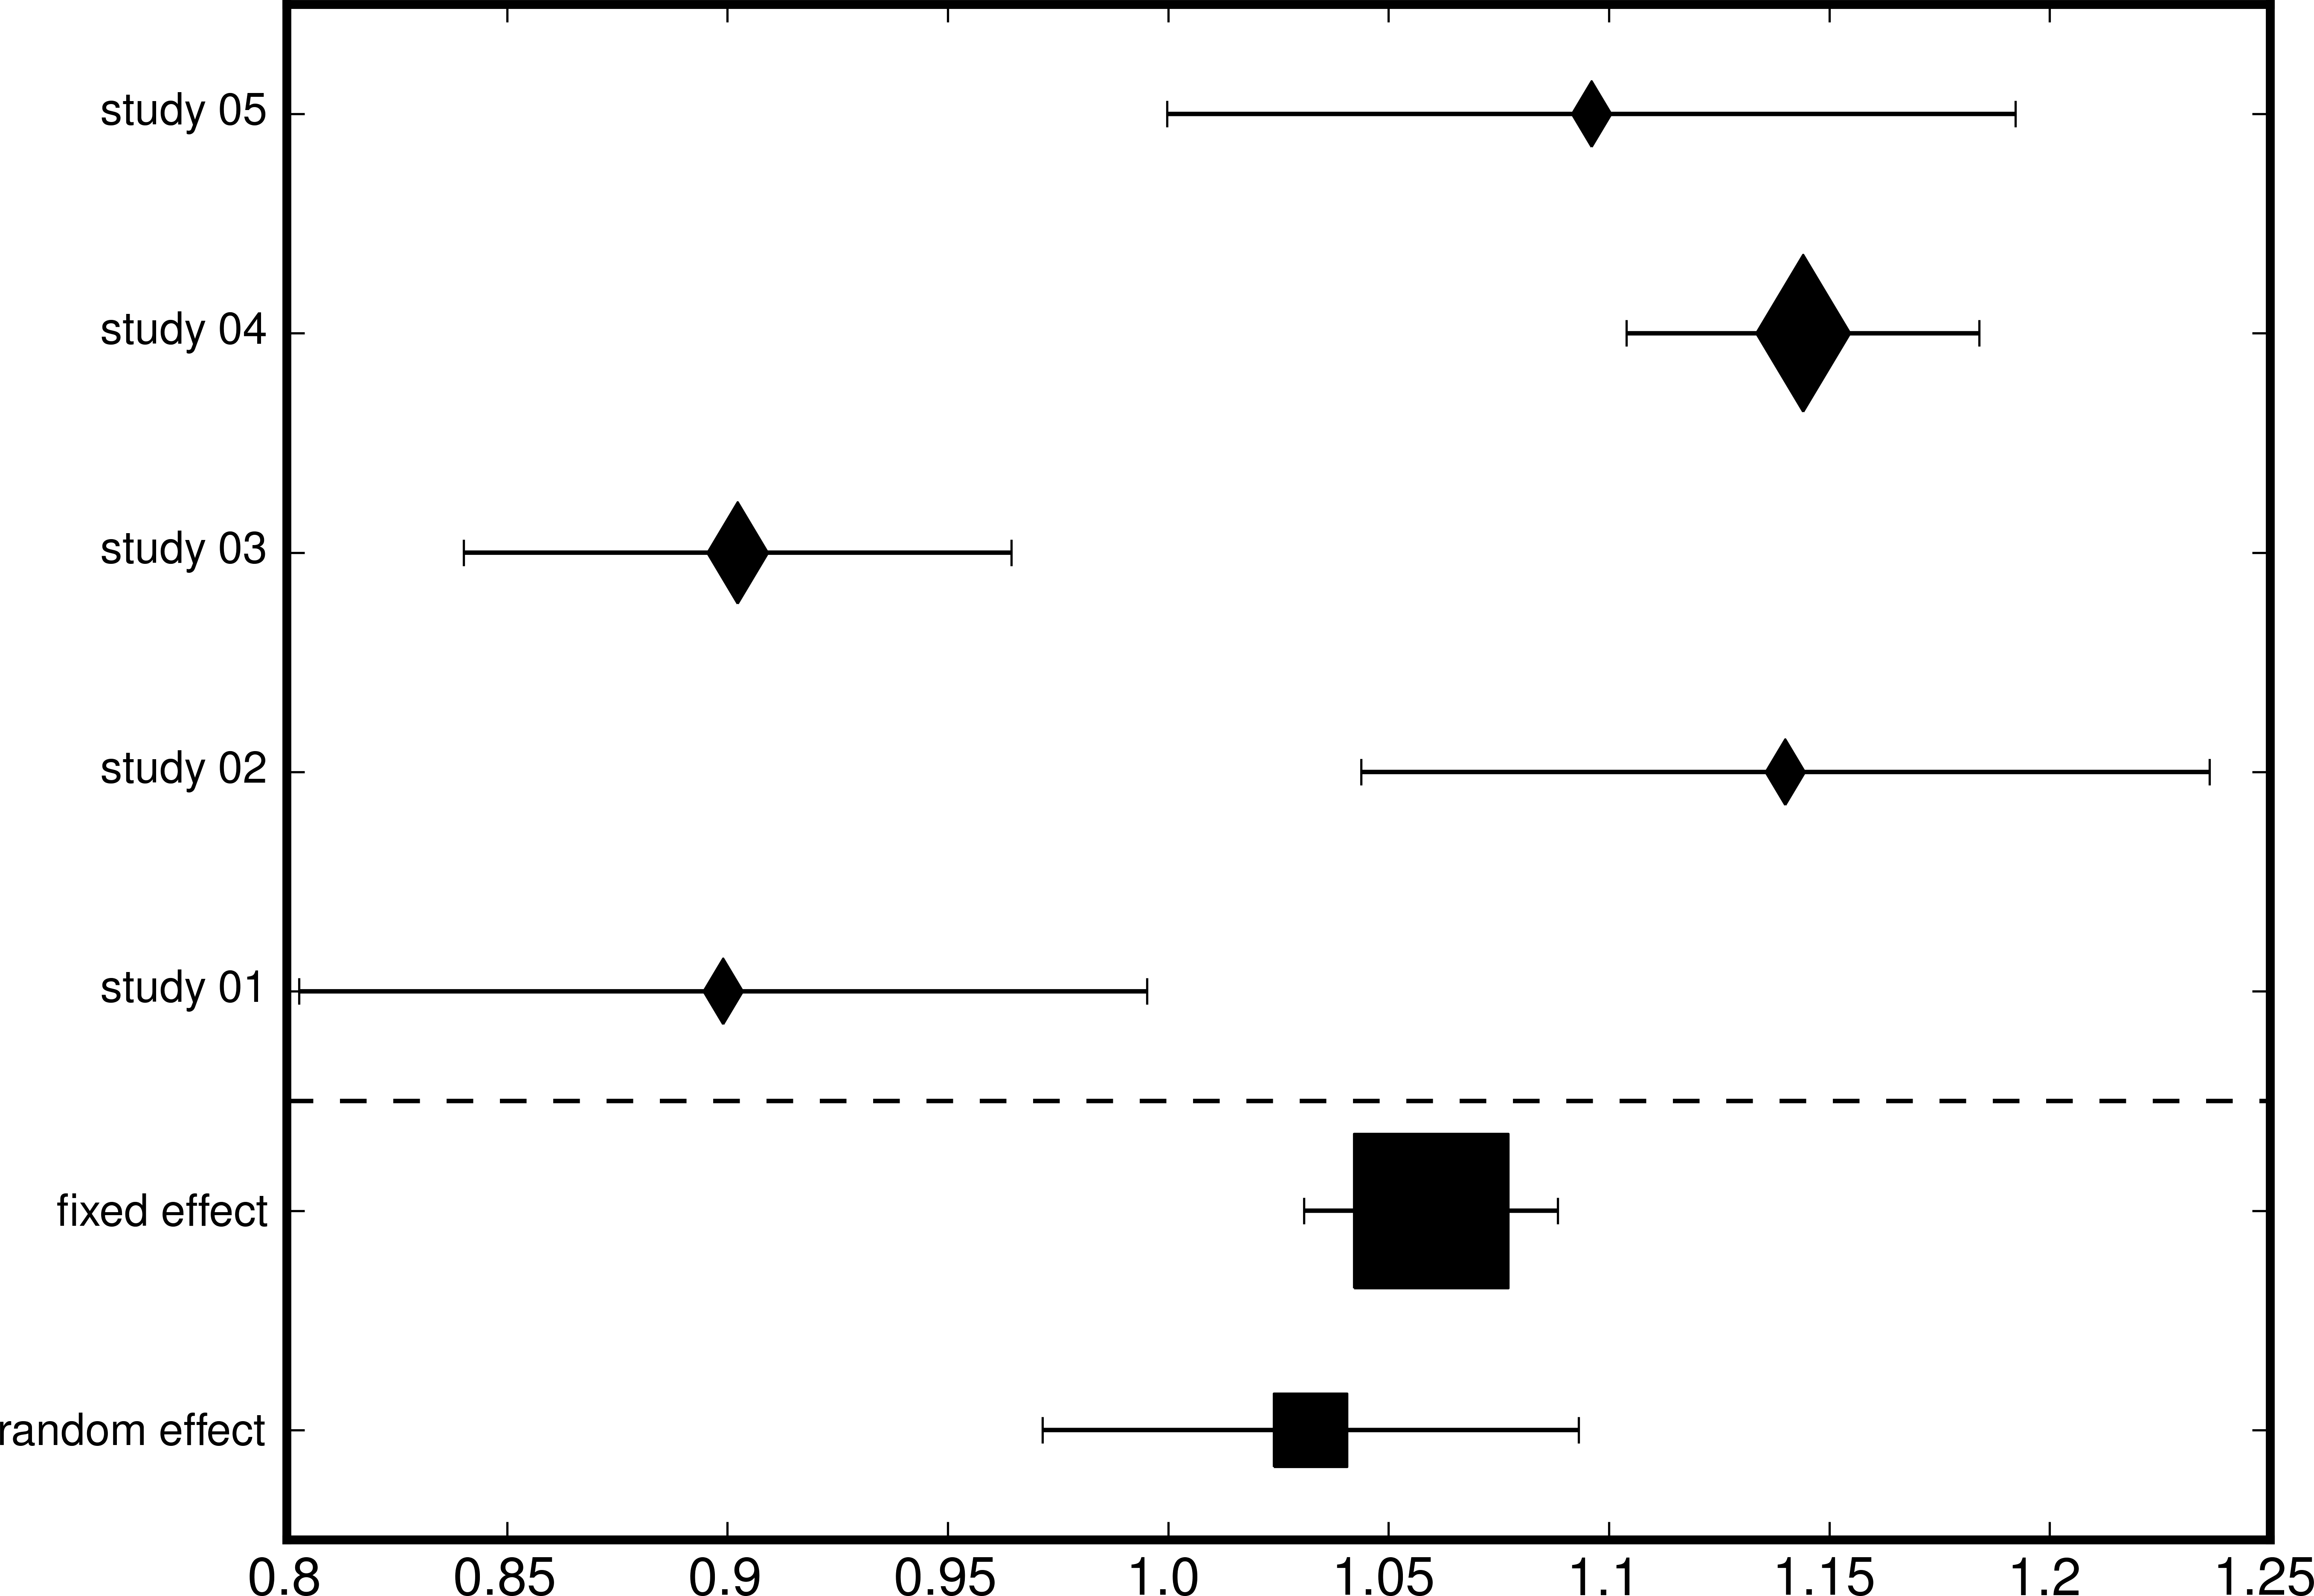
\includegraphics[width=.75\textwidth]{./images/rs9442372.png}
 \caption{Example forest plot for one particular marker showing how the more conservative random effect reflects the variance between studies. Note that the marker size (marker of the plot, not the GWAS) is inverse proportional to the standard error of that marker within a study or the meta-analysis.}
 \label{utilities:fig:forest_plot}
\end{figure}

\section{Switching Genotypes}

Occasionally studies may differ in there designation of effect and reference or other alleles for many markers. In this case \textsc{yamas} will refuse to consider these markers as valid, because the meta-analysis requires reliable effect directions and automatic corrections (described in paragraph \ref{algo:alleles}) cannot be accomplished if the genotypes aren't the same.

In this case the \verb+swith_markers+-script can change the genotypes of particular markers according to a reference. The script is invoked like

\begin{lstlisting}[style=shell]
$ <path>/switch_markers --configfile    <configuration file> \
                        --referencefile <the study file which \
                       genotypes should serve as a reference> \
                        --wrongfile     <the study file which \
                       genotypes should be corrected>
\end{lstlisting}

The command can be typed on one line, the \verb+\+ omitted.

Currently (as of \textsc{yamas} version 0.5) two cases are considered:
\begin{itemize}
 \item The genotypes are identical - hence, the genotypes in \verb+wrongfile+ are left untouched.
 \item The genotypes are each others complements - here, the genotypes in \verb+wrongfile+ for the respective marker are changed to their complements.
\end{itemize}

\section{Transforming \texttt{.vcf}-Files to Plink Compatible Format}

While \textsc{yamas} provides refrence files for the ``proxy-algorithm'' (see paragraph \ref{algo:fillwithproxies}, own reference files can be generated (see paragraph \ref{algo:own_refernce_files}). For this purpose Plink \citep{Purcell2007} compatible files are needed. Some projects, e.\,g. the 1000 genomes project, provide their data in the \texttt{vcf}-format. To transform \texttt{.vcf}-files into Plink \texttt{tped/tfam} file tuples, please have a look at the \texttt{vcf2tped} script in the utility directory of your download.  

\section{More Utilities?}

Obviously we cannot provide solutions for all imaginable problems which may come with meta-analysis. If you encounter a so far unsolved problem, please contact us: Either provide a general solution for that problem as a script (not necessarily Python) -- your name will be mentioned! -- or ask us for help, such that we can provide a script to solve your problem (in more complex cases we might ask for co-authorship).



% $Rev: 864 $
% $LastChangedDate: 2012-01-23 10:32:16 +0100 (Mo, 23 Jan 2012) $ 
% $Author: meesters $ 
\chapter{Shorties}

This chapter is a loose, non-comprehensive collection of useful tools for \verb+yamas+-users.

Sorting files numerically the UNIX way:
\begin{lstlisting}[style=shell]
$ sort -nk <column> file > sorted file
\end{lstlisting}

There is no need to unzip those really big reference files, used in \verb+yamas+, as
unzipping works on the fly without writing on the disk the unzipped file:
\begin{lstlisting}[style=shell]
$ gunzip -c <path to gzipped file> | <command, e.g. grep>
\end{lstlisting}

% $Rev: 891 $
% $LastChangedDate: 2012-05-08 14:23:42 +0200 (Di, 08 Mai 2012) $ 
% $Author: meesters $ 
\chapter[Development]{\textsc{yamas} -- Development}

The following chapters are intended for developers of \textsc{yamas}. You are most welcome to participate! Contributions may not only be code-based: Any bug report, hint on how to improve the manual, or feature request is welcome.

\section{How to retrieve a working copy of \textsc{yamas}}

\textsc{yamas} is not anonymous! Therefore you need an account for our repository. Every contributing developer is welcome, please do not hesitate contacting us for a login.

A checkout requires \textsc{subversion} (see \url{subversion.tigris.org}). This versioning system is available for (almost) every operating system. Please contact your local administrator, if you don't know how the program can be installed.

A first checkout can be done as follows:

\begin{lstlisting}[style=shell]
svn co --username <username> \
 svn+ssh://<username>@131.220.23.67/daten/svnrep/yamas <path>
\end{lstlisting}

You can ommit the \verb+\+-sign and type everything in one line. Everything between \verb+< ... >+ should be replace by the appropriate username and path. \verb+path+ can be any path you like, including the current working directory (\verb+.+).

\alert{Subsequently only use \texttt{svn update} after you did the first checkout. Subversion checkouts should be performed once and only once per working directory!}

\section{Building the development version}
\textsc{yamas} uses \texttt{scons} (see \url{www.scons.org}) as a build system (UNIX's \texttt{make} is the most well-known counterpart). In order to build a svn download just type
\begin{lstlisting}[style=shell]
$ cd your-yamas-download-path
$ scons
$ scons -c # will clean up after building
\end{lstlisting}
\texttt{scons} is available for download on the \texttt{scons} web page. However, many systems provide packages for \texttt{scons}. Please consult your sys-admin if in doubt.

\section{Colorized Compiler Output}

The \textsc{yamas} \texttt{SConstrust}-file prepares for using \texttt{colorgcc} (see \url{http://schlueters.de/colorgcc.html}). Using \texttt{colorgcc} is optional, if a colorized compiler output is appreciated you will have to install \texttt{colorgcc} locally in your \texttt{\$PATH}.

\section{Packing a Release Version}
\alert{Update the \texttt{yamas} version in the \texttt{SConstrust}-file, first. \texttt{yamas} follows the GNU version numbering scheme: major.minor.revision .}

Prior to packing a release, please update the repository first:
\begin{lstlisting}[style=shell]
$ svn update
\end{lstlisting}
This is because \texttt{yamas} can report is version and revision number and updating first makes sure that users reporting bugs can be sure about the release.

Typing
\begin{lstlisting}[style=shell]
$ scons --static
# and subsequently !!!
$ scons --pack_release
\end{lstlisting}
will create a directory called \texttt{dist} with the appropriately packed files for the current system. 

Right now, there is a variable called \verb+file_list+ in the \texttt{SConstrust}-file which describes the files to be packed, like this:
\begin{lstlisting}[style=python]
 file_list = [('../yamas', './yamas_%s/yamas' % VERSION),
                 ('../LICENSE', './yamas_%s/LICENSE' % VERSION),
                 ('../trunk/data/yamas.cfg', 
                      './yamas_%s/examples/yamas.cfg' % VERSION),
                 ('../trunk/doc/Manual.pdf', 
                      './yamas_%s/doc/Manual.pdf' % VERSION)]
\end{lstlisting}
Read this line as follows: The first item or string in each line is the file to be packed, the second the path where it should end after unpacking/-taring/-zipping the packed files. Please feel free to add all files, which might be useful for potential users after download.

The \texttt{VERSION} parameter is just the version string, which will be used for naming the download directory as a unique identifier of the \textsc{yamas} version.

A file containing the md5 sums for all produced files is written out, too.

\subsection{Supplying the Download Server with Large Files}

Our download server is capable of handling pretty big files, yet \texttt{yamas} reference files can be too be for the CMS. So, please copy any big file directly to:
\verb+/srv/www/htdocs/yamas/dm_documents+
at 131.220.23.75. An account can be created upon request.

\section{Building a Debug Version}

Invoking \textsc{scons} like
\begin{lstlisting}[style=shell]
$ scons --debug_build
\end{lstlisting}
Will compile and link with \verb+-g+, \verb+-pg+, and \verb+-DDEBUG+ flags. The first two flags enable using the GNU debugger (by writing a file named \verb+gmon.out+ when \textsc{yamas} runs). The third flag turns internal error handling routines of \textsc{yamas} off.

\section{Selecting Compilers}

For an explicit compiler seletion try:
\begin{lstlisting}[style=shell]
$ scons --compiler=g++-4.4
\end{lstlisting}
for instance.

\section{Parallel Builds with Scons}

Like the infamous GNU \verb+make+ tool, \textsc{scons} allows using the \verb+-j+ option to build an application in parallel:  
\begin{lstlisting}[style=shell]
$ scons -j <number of parallel compiler calls>
\end{lstlisting}

\section{Including Sandboxed Code}

If a Developer wants to create sandbox code, that is code which should not turn up in productive versions of the program until completion of that code, the code in question can be framed with preprocessor guards like this:
\begin{lstlisting}[style=C++]
#ifdef SANDBOX
// your sandbox code here
#endif
\end{lstlisting}
This guard can be applied to entire \verb+cpp+-files.

Issuing the \verb+--sandbox+-flag to scons will turn the \verb+SANDBOX+-preprocessor variable on.


\section{Other Options}
\begin{lstlisting}[style=shell]
$ scons --help 
\end{lstlisting}
will list a bundle of additional options we included to ease the \textsc{yamas} development.

\section{Used Libraries}

\subsection{\texttt{OpenMP}}

\textsc{yamas} uses \texttt{OpenMP} to spawn threads on shared memory systems. This way some algorithms can reach a tremendous speed-up. Please install the appropriate header for your system using the system's packaging tools.

\texttt{gcc} from version 4.4 on will support \texttt{OpenM}P 3.0. We recommend using gcc as the compiler. However, necessary instructions for other compilers are linked here: \url{http://openmp.org/wp/openmp-compilers/}.

\subsection{\texttt{boost}}

\textsc{yamas} makes heavy use of \texttt{boost} (see \url{http://www.boost.org/} for download and instructions). In order to ease the installation process, here a shortcut for Unix-like systems:

\begin{lstlisting}[style=shell]
$ # need to install MPI library
$ # Debian and Ubuntu users:
$ sudo apt-get install lam4-dev libopenmpi-dev
\end{lstlisting}
\textbf{Or} subversion source code checkout:
\begin{lstlisting}[style=shell]
svn co http://svn.boost.org/svn/boost/trunk boost-trunk
\end{lstlisting}
\alert{boost checkout is anonymous. See \url{http://www.boost.org/users/download/}. Subsequently only use \texttt{svn update} after you did the checkout. Subversion checkouts should be performed once and only once per working directory!}

Installation:
\begin{lstlisting}[style=shell]
$ cd your-boost-download-directory
$
$ ./bootstrap.sh --help # shows configuration options
$ ./bootstrap.sh
$ ./bjam # this will take a while
$ # and finally
$ sudo ./bjam --with-regex install
\end{lstlisting}

If you don't have administrator rights:
\begin{lstlisting}[style=shell]
$ ./bootstrap.sh --prefix=path/to/installation/prefix
$ ./bjam
$ ./bjam --with-regex install
\end{lstlisting}

The \verb+--with-regex+-flag is important!

\alertv{\textbf{Troubleshooting:}

\begin{itemize}
 \item \textsc{yamas} does not link against \texttt{boost::iostreams}? One reason might be that this particular library did not compile. In this case try setting the environment variable \texttt{NO\_BZIP2} to 1 and re-run \texttt{bjam}. For bash-like shell the command is ``\texttt{export NO\_BZIP2=1}''.
 \item \textsc{yamas} does not link at all? Please set the enviroment variable \texttt{LIBRARY\_PATH} to the appropriate path. Consult your local administrator if you don't know how.
\end{itemize}

}

\subsection{\texttt{zlib}}
\textsc{yamas} uses \verb+boost::iostreams+ to decompress zipped files on the fly. In order to compile \verb+zlib+-headers are required. See \url{www.zlib.net} for detail and / or consult your systems packaging system.

\section{Programming Standards}

The purpose of these standards is to provide a consistent, professional look for the source code. Deviations from the general rules below are acceptable if they enhance the readability of the code.

That being said, it's perfectly ok, if you do not adhere to the following standards -- as long as the code stays understandable.

\begin{itemize}
 \item Tabs: There should be no embedded tab characters in the source code.
 \item Indentation: Normal indentation should be 4 spaces.
 \item Braces should start directly after an opening statement -- separated with a space\footnote{This is the preferred style of one developer (C. Meesters).}. Example:
\begin{lstlisting}[style=C++]
for (i = 1; i = 10; i++) {
   if (test) {
      block of code
   } 
}
\end{lstlisting}
\item Braces should start one line below an opening statement\footnote{This is the preferred style of a second developer (T. Becker).}. Example:
\begin{lstlisting}[style=C++]
for (i = 1; i = 10; i++)
{
   if (test) {
      block of code
   } 
}
\end{lstlisting}
 \item Pragmas may follow yet a different bracing style:
\begin{lstlisting}[style=C++]
 #pragma omp critical
 {
 some_vector.push_back(item)
 }
\end{lstlisting}
Justification: pragmas are a special compiler directive and -- if braces are needed usually followed by short code segments, which should be easily ``spottable'' / distinguished by the reader.
 \item Braces are not required for one line conditions or very simple for loops\footnote{Also disliked by one of the developers.}. 
\begin{lstlisting}[style=C++]
if (test) return;
\end{lstlisting}
 \item Variable declarations:
 \begin{enumerate}
   \item Each variable declaration should be in a separate line.
   \item Pointers and references should be associated with the variable name, not the type. That is, use the K\&R and not the Strostrup style.
   \item If reasonable, line up variable names and any equal signs for assignments.
   \item Group variable definitions of the same type together.
 \end{enumerate}
 \begin{lstlisting}[style=C++]
int     x;
int     range;
string* lbl_a;
double  temperature = 72.0;
double  y           = 1.2;
\end{lstlisting}
 \item Class variables. Try to minimize these. When necessary, make public only when truly needed. 
 \item Spacing:
 \begin{enumerate}
   \item There should not be a space between a function name and the opening parenthesis.
   \item There should be a space after a programming construct ( if, for, while, etc. )
   \item There should be \textbf{no} space after an opening parenthesis or bracket and before a closing parenthesis or bracket.
   \item There should be a space around operators such as !, =, <=, etc.
 \end{enumerate}
 \begin{lstlisting}[style=C++]
for (i = 0; i < 10; i++) {
      x[i] = function(a, b, c);    
  }
 \end{lstlisting}
 \item Try to keep line lengths to 80 characters or less. Occasionally exceeding 80 characters is OK if a line break would detract from the overall readability.
 \item If arguments to a function don't fit nicely on one line, split it like this:
 \begin{lstlisting}[style=C++]
int lots_of_args(int an_integer, long a_long, short a_short,
                 double a_double, float a_float )
 \end{lstlisting}
 \item Line things up when it makes sense.
\end{itemize}







\clearpage\pagebreak
\addcontentsline{toc}{chapter}{Bibliography}

\bibliographystyle{chicago}	% (uses file "plain.bst")
\bibliography{./literature}

\end{document}
